\pdfinfoomitdate=1
\pdftrailerid{}
\pdfsuppressptexinfo=-1
\documentclass[sigplan,review,anonymous,pbalance]{acmart}

% === Layout Tuning Block ===
\usepackage{booktabs}
\usepackage{amsmath}
\usepackage{graphicx}
\usepackage{microtype}
\usepackage[htt]{hyphenat}
\raggedbottom
\emergencystretch=2em
\setlength{\partopsep}{0pt}
\setlength{\textfloatsep}{6pt plus 1pt minus 1pt}
\setlength{\dbltextfloatsep}{7pt plus 1pt minus 1pt}
\setlength{\floatsep}{5pt plus 1pt minus 1pt}
\setlength{\dblfloatsep}{6pt plus 1pt minus 1pt}
\setlength{\abovecaptionskip}{3pt}
\setlength{\belowcaptionskip}{1pt}
\renewcommand{\topfraction}{0.92}
\renewcommand{\dbltopfraction}{0.92}
\renewcommand{\textfraction}{0.08}
\settopmatter{printacmref=false, printfolios=true}
\renewcommand\footnotetextcopyrightpermission[1]{}
\acmConference[Agent Skills '27]{Agent Skills Workshop (ACM CAIS '27)}{2027}{TBA}
\acmYear{2027}
\AtBeginDocument{%
  \hypersetup{pdfauthor={},pdfcreator={},pdfproducer={}}%
  \setlength{\abovedisplayskip}{5pt plus 1pt minus 1pt}%
  \setlength{\belowdisplayskip}{5pt plus 1pt minus 1pt}%
  \setlength{\abovedisplayshortskip}{3pt plus 1pt minus 1pt}%
  \setlength{\belowdisplayshortskip}{3pt plus 1pt minus 1pt}%
}
\renewcommand\showeprint[2][]{arXiv:#2.}
\providecommand{\tightlist}{%
  \setlength{\topsep}{3pt}\setlength{\itemsep}{1pt}\setlength{\parskip}{0pt}}
% === End Layout Tuning Block ===

\title[PaperOEGM: Composable Zero-API-Key Agent Skills]{PaperOEGM: Composable Zero-API-Key Agent Skills with Deterministic Provenance Verification and Fresh-Context Peer Review}

\author{Anonymous Author(s)}
\affiliation{%
  \institution{Anonymous Institution}
  \country{Anonymous Country}
}
\email{anonymous@example.edu}

\begin{document}

\begin{abstract}
Packaging multi-stage scientific workflows as reusable Agent Skills (\texttt{SKILL.\allowbreak{}md} packages) exposes three coupled engineering failure modes: prompt context bloat and packaging defects across coding-agent harnesses, unverified provenance drift between experimental logs and manuscript claims, and security or anonymity leaks from untrusted literature records and external LaTeX templates. Existing automated paper-writing systems rely on external Large Language Model (LLM) API keys, monolithic pipelines, or same-context self-review that cannot reliably self-correct reasoning. We present \textbf{PaperOEGM}, a zero-API-key Agent Skills plugin packaged for Antigravity (live-verified end to end), Claude Code (packaging-validated), and Codex (structurally packaged). PaperOEGM separates \emph{deterministic mechanical verification} from \emph{fresh-context semantic critique} across three layers: (1) ten progressive-disclosure skills (3,466--4,526 bytes each, at most 63 lines) guarded by explicit human gates and SHA-256 digest drift tracking; (2) a zero-dependency Python standard-library verifier (\texttt{po\_\allowbreak{}tools.\allowbreak{}py}) checking citation snapshots, non-synthetic provenance, inline run-to-metric matching, Markdown-to-LaTeX parity, double-blind hygiene, and archive safety; and (3) five flat single-level read-only critic subagents paired with paranoid LaTeX compilation. Empirically, PaperOEGM cuts median active-stage prompt context by 82.16\% (97.14\% startup index reduction) with 0 packaging defects and 100.0\% deterministic ZIP SHA-256 parity; detects 100.0\% of 80 faults/seed with 0.0\% false positives on our author-constructed 120-workspace PO-FaultBench (108.20 ms/workspace) while exposing 0.0\% deterministic recall on 20 adversarial evasions/seed; scales to 120 citations in 268.55 ms with 87.96\% ledger offloading and 0 identity leaks across three compiled venues---uncovering an upstream TeX Live 2026 \texttt{openin\_\allowbreak{}any=p} read-sandbox no-op; and recovers 100.0\% of planted semantic flaws across three seeded domain manuscripts via 15 live read-only critic invocations with 0 workspace mutations.

\end{abstract}

\keywords{Agent Skills, Coding Agents, Scientific Provenance, Automated Peer Review, LaTeX Security}

\maketitle

\section{Introduction}\label{sec:intro}

The open \texttt{SKILL.\allowbreak{}md} format packages procedural instructions, helper scripts, and reference templates into progressive-disclosure folders loaded on demand by Large Language Model (LLM) coding agents \citep{destefanis2026gitskills, xu2026agentskills}. Yet empirical audits reveal widespread fragility. Mining 3,797,117 public \texttt{SKILL.\allowbreak{}md} files across 282,200 GitHub repositories, \citet{destefanis2026gitskills} note that natural-language skills lack compilers, type checkers, or package verifiers. Across 138,133 public skills, \citet{zhang2026reusable} find 91.8\% contain at least one defect---chiefly bloated instruction bodies and broken metadata---while SkillsBench \citep{li2026skillsbench} shows across 87 tasks and 18 model-harness configurations that curated skills lift pass rates from 33.9\% to 50.5\% (+16.6 percentage points) and focused skills (at most three modules) outperform larger exhaustive bundles. Simultaneously, security studies document high community vulnerability rates \citep{xu2026agentskills, badhe2026skillsecurity}, up to 80\% attack success rate (ASR) on skill-file prompt injections \citep{schmotz2026skillinject}, and semantic supply-chain hijacking \citep{saha2026underhood}.

Research-to-paper authoring stresses all of these weaknesses simultaneously, spanning literature review, experimental execution, visualization, drafting, peer review, and double-blind LaTeX compilation. Existing automated scientific writers---The AI Scientist \citep{lu2024aiscientist}, The AI Scientist-v2 \citep{yamada2025aiscientistv2}, CycleResearcher \citep{weng2024cycleresearcher}, and PaperOrchestra \citep{song2026paperorchestra}---operate as standalone automated pipelines outside interactive coding-agent skill ecosystems. Porting full scientific authoring into interactive coding harnesses exposes four unresolved challenges:

\begin{enumerate}
\def\labelenumi{\arabic{enumi}.}
\tightlist
\item
  \textbf{Context bloat and harness lock-in:} Monolithic playbooks exceed host loader ceilings (e.g., Antigravity's observed 24 KB / 24,000-byte skill limit) and waste prompt context across inactive stages.
\item
  \textbf{Silent provenance and conversion drift:} Without mechanical checks linking manuscript metrics to canonical run logs and citations to saved snapshots, drafting and Markdown-to-LaTeX export silently introduce fabricated decimals, synthetic dry-run leaks, or dropped equations and labels.
\item
  \textbf{Intrinsic self-review bias:} Because LLMs cannot reliably self-correct reasoning without external feedback \citep{huang2024selfcorrect}, same-context self-review misses missing ablations, claim-vs-source contradictions, and prose anonymity leaks.
\item
  \textbf{Scientific supply-chain vectors:} Authoring consumes untrusted abstracts, PDFs, and external conference LaTeX archives---exposing agents to indirect prompt injection \citep{greshake2023indirect}, Zip Slip traversal, LaTeX \texttt{\textbackslash{}write18}/\allowbreak{}\texttt{\textbackslash{}input\{\textbar{}...\}} shell pipes, arbitrary writes, and PDF metadata leaks.
\end{enumerate}

We present \textbf{PaperOEGM} (Paper Orchestra + Elephant-Goldfish Model, adopting the Elephant-Goldfish metaphor of durable workspace memory paired with fresh-context review \citep{google2026egm}), a zero-API-key Agent Skills plugin packaged for Antigravity (live-verified end to end), Claude Code (CLI packaging-validated), and Codex (structurally packaged). PaperOEGM uses zero external LLM API keys and zero third-party Python dependencies for its core verifier (\texttt{po\_\allowbreak{}tools.\allowbreak{}py}), requiring optional \texttt{matplotlib} only for Stage 5 plotting. Its architecture strictly separates \emph{deterministic mechanical verification} from \emph{fresh-context semantic critique} across three layers (Figure~\ref{fig:architecture}): ten budgeted skills (\texttt{\textless{}=\ 12\ KB}, \texttt{disable-model-invocation:\ true}), a standard-library CLI verifier over single-source \texttt{paper\_\allowbreak{}state.\allowbreak{}json}, and five flat single-level read-only critics paired with paranoid LaTeX compilation.

\begin{figure*}[t]
\centering
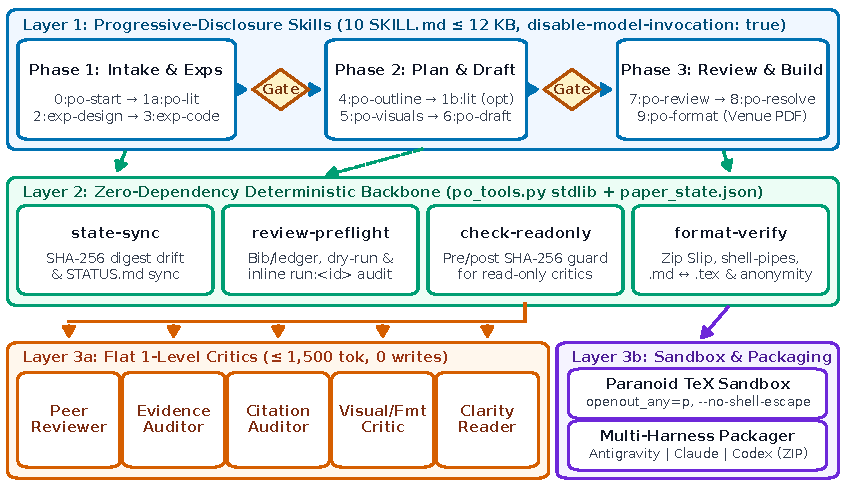
\includegraphics[width=0.88\textwidth]{figures/fig_architecture.pdf}
\caption{PaperOEGM three-layer architecture: progressive-disclosure skills with human checkpoint gates (Layer 1), zero-dependency stdlib verifier backbone (Layer 2), and flat 1-level read-only critics paired with paranoid LaTeX sandboxing and deterministic multi-harness packaging (Layer 3).}
\label{fig:architecture}
\end{figure*}

We make five contributions:

\begin{itemize}
\tightlist
\item
  \textbf{Multi-harness zero-API-key architecture (Section~\ref{sec:method}):} A 10-skill progressive-disclosure graph, single-source \texttt{paper\_\allowbreak{}state.\allowbreak{}json} digest tracker, safe bash experiment contract, flat 1-level read-only critic topology, paranoid TeX wrapper, and deterministic ZIP packager.
\item
  \textbf{PO-FaultBench and deterministic boundaries (Section~\ref{sec:exp-rq1}):} On an author-constructed 120-workspace fault suite (80 faults + 40 hard negative controls per seed, five seeds), \texttt{po\_\allowbreak{}tools.\allowbreak{}py} achieves 100.0\% recall and 0.0\% false-positive rate (FPR) in 108.20 ms/workspace vs.~6.25\% (Compiler-Only) and 87.5\% (No-Inline-Provenance), while recording 0.0\% recall on 20 adversarial evasions/seed---delineating where native sandboxes and semantic critics are mandatory.
\item
  \textbf{Context economics and build determinism (Section~\ref{sec:exp-rq2}):} PaperOEGM reduces median active-stage context by 82.16\% (97.14\% startup index reduction) vs.~monolithic loading, keeps 81.14\% headroom below Antigravity's 24 KB (24,000-byte) ceiling (where public EGM \citep{google2026egm} reaches 24,257 bytes), passes \texttt{claude\ plugin\ validate} with 0 defects, and achieves 100.0\% ZIP SHA-256 parity.
\item
  \textbf{Scalability and paranoid TeX containment (Section~\ref{sec:exp-rq3}):} Across 20--120 citations and 5--30 runs, all four verifier commands run in 266.00--268.55 ms, offload 87.82\%--87.96\% of raw metadata from \texttt{citation\_\allowbreak{}ledger.\allowbreak{}json}, compile three double-blind venues with 0 identity leaks, and block obfuscated shell escapes and parent-directory writes while exposing an upstream TeX Live 2026 \texttt{openin\_\allowbreak{}any=p} no-op regression.
\item
  \textbf{Live hybrid semantic critique (Section~\ref{sec:exp-rq4}):} Across three seeded domain manuscripts (30 planted flaws), deterministic checks catch 100.0\% of mechanical flaws in 91.71 ms but 0.0\% of semantic flaws (50.0\% total), whereas 15 live Antigravity read-only critics recover 100.0\% of semantic flaws with 0.0 clean-control FPs, 0 workspace mutations, and outputs within 1,500 tokens. Limitations are detailed in Section~\ref{sec:limitations}.
\end{itemize}

\section{Related Work}\label{sec:related}

PaperOEGM intersects four areas: Agent Skill packaging, skill security, automated paper writing, and fresh-context LLM review.

\subsection{Agent Skill Packaging and Context Economics}\label{agent-skill-packaging-and-context-economics}

Agent Skills package Markdown (\texttt{SKILL.\allowbreak{}md}) procedures with optional scripts and references loaded via progressive disclosure \citep{xu2026agentskills, destefanis2026gitskills}, extending Agent-Computer Interface (ACI) insights that structured interfaces govern coding-agent reliability \citep{yang2024sweagent}. Large-scale audits show weak packaging hygiene: \citet{destefanis2026gitskills} catalog 3,797,117 \texttt{SKILL.\allowbreak{}md} files (1,877,981 unique contents) across 282,200 repositories lacking static verifiers, and \citet{zhang2026reusable} find 91.8\% of 138,133 skills (20,556 repositories) have at least one defect, while confirming on a 20,000-skill test that valid metadata improves startup routing.

On utility, SkillsBench \citep{li2026skillsbench} (87 tasks, 8 domains, 18 model-harness pairs) shows curated skills raise average pass rates from 33.9\% to 50.5\% (+16.6 percentage points), with focused skills (at most three modules) outperforming larger exhaustive bundles. SkillTester \citep{wang2026skilltester} pairs baseline-vs.-with-skill execution with security probes. Closest in packaging philosophy is the open-source Elephant-Goldfish Model (EGM v0.1.1) \citep{google2026egm}, which packages fresh-context Goldfish reviewers across Antigravity, Claude Code, and Codex for software design docs. Unlike PaperOEGM, EGM lacks experiment safety, quantitative provenance, citation ledgers, and LaTeX sandboxing, and relies on a nested \texttt{synthesizer} subagent incompatible with non-nesting runtimes.

\subsection{Skill Security and Supply-Chain Auditing}\label{skill-security-and-supply-chain-auditing}

Because skills mix natural-language instructions and executable scripts, they amplify Indirect Prompt Injection \citep{greshake2023indirect}. Skill-Inject \citep{schmotz2026skillinject} (202 injection-task pairs spanning obvious to subtle context-dependent skill-file attacks) reports up to 80\% ASR on frontier LLMs, showing model scaling and naive input filters are insufficient without context-aware authorization. \citet{saha2026underhood} demonstrate \texttt{SKILL.\allowbreak{}md}-only semantic supply-chain attacks achieving up to 86\% retrieval win rate, 77.6\% paired-trial selection rate (over a 50\% baseline), and 36.5\%--100\% governance evasion. Surveying the ecosystem, \citet{xu2026agentskills} cite analyses finding 26.1\% of community skills vulnerable, while \citet{badhe2026skillsecurity} introduce SkillSec-Eval across 327 skills and a five-stage lifecycle (repository admission, semantic retrieval, planner selection, execution, skill evolution); \citet{lv2026structuredaudit} propose SkillGuard-Robust for cross-file auditing under semantics-preserving rewrites. Scientific authoring adds domain-specific vectors---untrusted conference LaTeX archives (Zip Slip, \texttt{\textbackslash{}write18}, \texttt{\textbackslash{}input\{\textbar{}...\}}), secret leaks in experiment logs, and double-blind PDF metadata leaks---which PaperOEGM directly targets.

\subsection{Automated Research and Fresh-Context Peer Review}\label{automated-research-and-fresh-context-peer-review}

Autonomous discovery pipelines---The AI Scientist \citep{lu2024aiscientist}, The AI Scientist-v2 \citep{yamada2025aiscientistv2}, and CycleResearcher \citep{weng2024cycleresearcher}---automate research loops and simulated review via external LLM APIs or post-trained weights. Yet PaperBench \citep{starace2025paperbench} (20 ICML 2024 Spotlight/Oral papers, 8,316 rubric items) shows the strongest autonomous agent achieves only a 21.0\% average replication score, reinforcing human-in-the-loop checkpoints. Decoupling writing from fixed pipelines, PaperOrchestra \citep{song2026paperorchestra} turns unstructured pre-writing materials into LaTeX manuscripts and visuals (+50\%--68\% literature review and +14\%--38\% overall win margins on 200-paper PaperWritingBench), while PaperBanana \citep{zhu2026paperbanana} automates academic illustrations via Vision-Language Models (VLMs) and image generation. However, PaperOrchestra does not package interactive pre-experiment coding-agent skills, a zero-dependency deterministic run-to-manuscript verifier, or double-blind archive/TeX checks.

Finally, \citet{huang2024selfcorrect} show LLMs cannot reliably self-correct reasoning without external feedback, whereas \citet{liang2024feedback} (3,096 Nature-family and 1,709 ICLR papers; 308 researchers) show independent LLM review matches inter-human overlap (30.85\%/39.23\% vs.~28.58\%/35.25\%), with 57.4\% finding feedback helpful while noting limitations. PaperOEGM combines deterministic external verification (\texttt{po\_\allowbreak{}tools.\allowbreak{}py}) with five fresh-context read-only critics to capture both advantages without mutating the drafting workspace.

\section{System Design}\label{sec:method}

PaperOEGM packages an end-to-end research-to-paper workflow across Antigravity, Claude Code, and Codex around four invariants: (1) budgeted progressive-disclosure skills with human gates, (2) zero-dependency deterministic verification over single-source state, (3) flat single-level read-only peer review, and (4) defense-in-depth build safety.

\subsection{Progressive-Disclosure Skill Graph and State Machine}\label{sec:method-skills}

PaperOEGM decomposes authoring into ten skills under \texttt{skills/\allowbreak{}po-*/\allowbreak{}SKILL.\allowbreak{}md} (\texttt{po-literature} runs in two passes: Stage 1a early survey and optional Stage 1b late refresh) across three phases (Figure~\ref{fig:architecture}, Layer 1):

\begin{itemize}
\tightlist
\item
  \textbf{Phase 1 (Intake \& Experiments):} Stage 0 \texttt{po-start} (routing, secret denylist, toolchain probe), Stage 1a \texttt{po-literature}, Stage 2 \texttt{po-exp-design} (falsifiable hypotheses, ablations, metric schema), and Stage 3 \texttt{po-exp-code} (safe bash runners, \texttt{\mbox{-{}-}dry-\allowbreak{}run} smoke checks).
\item
  \textbf{Phase 2 (Plan \& Draft):} Stage 4 \texttt{po-outline} (canonical run reconciliation, page budget), Stage 1b \texttt{po-literature} (optional), Stage 5 \texttt{po-visuals} (code-rendered plots, multimodal audit), and Stage 6 \texttt{po-draft} (modular Markdown with inline provenance tags).
\item
  \textbf{Phase 3 (Review \& Build):} Stage 7 \texttt{po-review} (preflight + five flat parallel read-only critics), Stage 8 \texttt{po-resolve} (reversible snapshots and three-bucket triage separating mechanical fixes, scientific decisions, and optional polish), and Stage 9 \texttt{po-format} (Pandoc export, paranoid LaTeX build, \texttt{pdfinfo} hygiene, post-compile PDF layout audit).
\end{itemize}

Guided by empirical skill-reuse findings \citep{zhang2026reusable, li2026skillsbench}, every \texttt{SKILL.\allowbreak{}md} is capped at \texttt{\textless{}=\ 250} lines and \texttt{\textless{}=\ 12,\allowbreak{}000} bytes (half of Antigravity's observed 24 KB / 24,000-byte skill limit), offloading shared rules into \texttt{execution\_\allowbreak{}instructions.\allowbreak{}md}, six protocols (\texttt{resources/\allowbreak{}protocols/}), and five review standards (\texttt{resources/\allowbreak{}review\_\allowbreak{}standards/}). Every skill declares \texttt{disable-model-invocation:\ true}, blocking unprompted transitions and enforcing single-select human checkpoints. Single-source \texttt{paper\_\allowbreak{}state.\allowbreak{}json} owns title, venue (\texttt{name}, \texttt{template\_\allowbreak{}year}, \texttt{submission\_\allowbreak{}mode}, \texttt{page\_\allowbreak{}limit\_\allowbreak{}main}), probed tools, and SHA-256 \texttt{input\_\allowbreak{}hashes}/\allowbreak{}\texttt{output\_\allowbreak{}hashes}, regenerating \texttt{STATUS.\allowbreak{}md} atomically on every sync.

Let \(B_{\text{mono}}\) be the monolithic sum of all ten \texttt{SKILL.\allowbreak{}md} files, \texttt{execution\_\allowbreak{}instructions.\allowbreak{}md}, six protocols, and five standards; \(B_{\text{stage}}(s)\) the active footprint of skill \(s\) (\texttt{SKILL.\allowbreak{}md} + \texttt{execution\_\allowbreak{}instructions.\allowbreak{}md} + protocols directly referenced by \(s\)); and \(B_{\text{idx}}\) the combined startup YAML frontmatter index. Per-stage context reduction \(R_{\text{ctx}}\) and startup index reduction \(R_{\text{idx}}\) are:

\begin{equation}
\begin{aligned}
R_{\text{ctx}} &= \left(1 - \frac{\operatorname{median}_{s} B_{\text{stage}}(s)}{B_{\text{mono}}}\right) \times 100\%, \\
R_{\text{idx}} &= \left(1 - \frac{B_{\text{idx}}}{B_{\text{mono}}}\right) \times 100\%
\end{aligned}
\label{eq:context-reduction}
\end{equation}

\hypertarget{sec:method-verifier}{%
\subsection{\texorpdfstring{Zero-Dependency Deterministic Verifier (\texttt{po\_\allowbreak{}tools.\allowbreak{}py})}{Zero-Dependency Deterministic Verifier (po\_tools.py)}}\label{sec:method-verifier}}

To supply zero-stochasticity external verification \citep{huang2024selfcorrect} without runtime \texttt{pip\ install}, PaperOEGM bundles \texttt{resources/\allowbreak{}scripts/\allowbreak{}po\_\allowbreak{}tools.\allowbreak{}py}, a 758-line Python 3.10+ standard-library CLI with four subcommands (Figure~\ref{fig:architecture}, Layer 2):

\begin{enumerate}
\def\labelenumi{\arabic{enumi}.}
\item
  \textbf{\texttt{state-sync}:} Atomically validates \texttt{paper\_\allowbreak{}state.\allowbreak{}json} (\texttt{tmp} + \texttt{os.\allowbreak{}replace}), probes local binaries (\texttt{pandoc}, \texttt{latexmk}/\allowbreak{}\texttt{pdflatex}, \texttt{bibtex}, \texttt{pdftoppm}, optional \texttt{matplotlib}), counts unresolved \texttt{TODO} or pending-run markers, and flags upstream-modified downstream stages \texttt{stale}.
\item
  \textbf{\texttt{check-readonly}:} Snapshots (\texttt{\mbox{-{}-}create}) and verifies (\texttt{\mbox{-{}-}verify}) SHA-256 digests of tracked files inside the workspace before and after read-only critic execution, exiting 1 on any added, modified, or deleted file.
\item
  \textbf{\texttt{review-preflight}:} Audits mechanical provenance before spawning critics: (i) extracts Pandoc (\texttt{{[}@key{]}}, \texttt{@key}) and LaTeX (\texttt{\textbackslash{}cite*\{key\}}) citations across \texttt{manuscript/\allowbreak{}sections/\allowbreak{}*.md}, enforcing 1:1 parity with \texttt{literature/\allowbreak{}references.\allowbreak{}bib} and \texttt{literature/\allowbreak{}citation\_\allowbreak{}ledger.\allowbreak{}json}, blocking \texttt{unverified\_\allowbreak{}needs\_\allowbreak{}human\_\allowbreak{}check}, and confirming \texttt{verified\_\allowbreak{}source} files exist under \texttt{literature/\allowbreak{}sources/}; (ii) blocks references to the isolated \texttt{dry\_\allowbreak{}run/} path, \texttt{is\_\allowbreak{}synthetic:\ true} runs, and unattested \texttt{user\_\allowbreak{}byo} runs while flagging \texttt{git\_\allowbreak{}dirty:\ true} as Major; and (iii) parses inline \texttt{\textless{}!\mbox{-{}-}\ run:\textless{}run\_\allowbreak{}id\textgreater{}\ \mbox{-{}-}\textgreater{}} markers, auditing every decimal token \(v\) (\(d\) fractional digits) in the following paragraph/table block against the flattened numeric set \(\mathcal{M}(r)\) of canonical \texttt{metrics.\allowbreak{}json}:

  \begin{equation}
\begin{aligned}
&|m - v| \le \epsilon(d) \;\lor\; \\
&\quad \bigl(0 \le m \le 1 \;\land\; |100m - v| \le \epsilon(d)\bigr), \\
&\quad \epsilon(d) = 0.55 \times 10^{-d}
\end{aligned}
\label{eq:decimal-match}
\end{equation}

  where the second disjunct permits \(0\text{--}1 \to \%\) scaling strictly for \(m \in [0, 1]\) and \(\epsilon(d)\) allows standard rounding. Restricting regex matching to decimal tokens (\texttt{\textbackslash{}d+\textbackslash{}.\textbackslash{}d+}) avoids false alarms on section or epoch integers, intentionally delegating integer-count auditing, metric-key swapping within unordered \(\mathcal{M}(r)\), unit-ambiguous \([0, 1]\) scaling, and untagged paragraphs to \texttt{po-evidence-auditor}.
\item
  \textbf{\texttt{format-verify}:} Scans \texttt{.zip}/\allowbreak{}\texttt{.tar.\allowbreak{}*} template archives for Zip Slip (\texttt{..}, leading \texttt{/}), symlinks/hardlinks, and active TeX shell pipes (\texttt{\textbackslash{}write18}, \texttt{\textbackslash{}immediate\allowbreak{}\textbackslash{}write18}, \texttt{\textbackslash{}input\{\textbar{}...\}}) after stripping \texttt{\%} comments; checks \texttt{.md}-to-\texttt{.tex} citation, \texttt{\textbackslash{}label\{\}}, and non-dimension decimal parity (filtering LaTeX units like \texttt{0.85\textbackslash{}linewidth}, \texttt{10.5pt}); parses TeX \texttt{.log}/\allowbreak{}\texttt{.aux} telemetry (undefined refs/cites, missing graphics, \texttt{Overfull\ \textbackslash{}hbox\ \textgreater{}\ 2pt}); and enforces double-blind hygiene across \texttt{.tex} body and \texttt{\%} comments (blocking \texttt{/\allowbreak{}Users/}, \texttt{/\allowbreak{}home/}, \texttt{C:\textbackslash{}Users\textbackslash{}}, GitHub URLs, \texttt{\textbackslash{}iclrfinalcopy}, \texttt{\textbackslash{}usepackage\{cvpr\}}).
\end{enumerate}

\subsection{Experiment Safety, Visuals, and Context Offloading}\label{sec:method-safety}

Stage 3 runners enforce \texttt{set\ -euo\ pipefail}, double-quoted paths, \texttt{WANDB\_\allowbreak{}MODE=offline}, non-git fallback (\texttt{git\_\allowbreak{}commit:\ "none"}, \texttt{git\_\allowbreak{}dirty:\ null}), secret/\texttt{\$HOME} redaction in logged \texttt{cmd}, crash-safe startup \texttt{run\_\allowbreak{}manifest.\allowbreak{}json} + \texttt{trap\ finalize\ EXIT}, atomic \texttt{metrics.\allowbreak{}json} (\texttt{\textless{}\ 10\ KB}), and \texttt{\mbox{-{}-}dry-\allowbreak{}run} isolation in \texttt{dry\_\allowbreak{}run/\allowbreak{}\textless{}run\_\allowbreak{}id\textgreater{}/} (\texttt{is\_\allowbreak{}synthetic:\ true}).

Stage 1 stores raw primary-source API snapshots in \texttt{literature/\allowbreak{}sources/\allowbreak{}\textless{}citekey\textgreater{}.json} and keeps only compact pointers plus 1--2 sentence summaries in \texttt{citation\_\allowbreak{}ledger.\allowbreak{}json}, giving ledger offload ratio \(R_{\text{off}} = (1 - S_{\text{led}} / (S_{\text{led}} + S_{\text{src}})) \times 100\%\) for non-citation stages while \texttt{po-citation-auditor} loads snapshots on demand. Stage 5 requires newly generated quantitative plots to load directly from canonical non-synthetic \texttt{metrics.\allowbreak{}json}/\allowbreak{}\texttt{series.\allowbreak{}csv} via version-controlled Python scripts (optional \texttt{matplotlib}, zero hardcoded arrays, zero generative raster tools on data), exporting colorblind-safe dual-encoded vector PDFs with stripped metadata plus high-DPI PNG previews verified visually.

\subsection{Flat Critics, Paranoid TeX Sandbox, and Multi-Harness Packaging}\label{sec:method-critics}

Stage 7 dispatches five stateless read-only personas (\texttt{agents/\allowbreak{}po-*.md}, \texttt{\textless{}=\ 6,\allowbreak{}000} bytes)---\texttt{po-peer-reviewer}, \texttt{po-evidence-auditor}, \texttt{po-citation-auditor}, \texttt{po-visual-format-critic} (Pass 1 figures + Pass 2 chunked 4--5 page PDF layout), and \texttt{po-clarity-reader}---\textbf{flat at depth one in parallel} (Figure~\ref{fig:architecture}, Layer 3a). Unlike EGM's nested \texttt{synthesizer} \citep{google2026egm}, flat dispatch avoids nesting failures on Antigravity and Claude Code Cowork, bounds each critic to 1,500 output tokens, and logs a 4-state \texttt{Reviewer\ Status} table (\texttt{completed}, \texttt{skipped\_\allowbreak{}not\_\allowbreak{}applicable}, \texttt{carried\_\allowbreak{}forward}, \texttt{not\_\allowbreak{}run}); Claude Code adapters (\texttt{.claude-plugin/\allowbreak{}agents/\allowbreak{}po-*.md}) restrict \texttt{tools:} strictly to \texttt{Read,\allowbreak{}\ Grep,\allowbreak{}\ Glob}.

Because static regexes miss macro-obfuscated TeX escapes (e.g., \texttt{\textbackslash{}csname\ write18\textbackslash{}endcsname}), Stage 9 wraps compilation with paranoid flags (\texttt{openin\_\allowbreak{}any=p\ openout\_\allowbreak{}any=p\ pdflatex\ \mbox{-{}-}no-\allowbreak{}shell-escape}, where \texttt{p} requests paranoid mode disallowing dotfiles and parent directories), strips identity metadata via \texttt{\textbackslash{}hypersetup\{pdfauthor=\{\},\allowbreak{}pdfcreator=\{\},\allowbreak{}pdfproducer=\{\}\}}, and checks \texttt{pdfinfo}. As Section~\ref{sec:exp-rq3} verifies, \texttt{\mbox{-{}-}no-\allowbreak{}shell-escape} and \texttt{openout\_\allowbreak{}any=p} hold on TeX Live 2026 while \texttt{openin\_\allowbreak{}any=p} became an upstream no-op. Finally, \texttt{scripts/\allowbreak{}pack\_\allowbreak{}plugin.\allowbreak{}py} synchronizes all five manifests and emits deterministic ZIP bundles (fixed \texttt{1980-01-01} timestamps, sorted traversal) across Antigravity, Claude Code, and Codex.

\section{Experimental Evaluation}\label{sec:experiments}

We evaluate PaperOEGM across four research questions: deterministic fault detection (\textbf{RQ1}), multi-harness packaging and context economics (\textbf{RQ2}), verification scalability and paranoid TeX containment (\textbf{RQ3}), and live hybrid semantic critique (\textbf{RQ4}). RQ1--RQ3 execute locally on CPU without external LLM API keys (Python 3.12.8, TeX Live 2026, \texttt{pandoc}, \texttt{pdfinfo}, Claude Code CLI 2.1.328); RQ4 runs the deterministic baseline on CPU and dispatches 15 live read-only critics on Antigravity (Gemini 4). All runs execute against an unmodified plugin codebase (\texttt{git\ diff} outside \texttt{paper\_\allowbreak{}workspace/} is empty; resolution-phase workspace updates carry recorded \texttt{git\_\allowbreak{}dirty} attestations) and write strictly non-synthetic outputs (\texttt{is\_\allowbreak{}synthetic:\ false}) registered in \texttt{experiments/\allowbreak{}provenance\_\allowbreak{}index.\allowbreak{}json}, keeping smoke checks segregated in \texttt{dry\_\allowbreak{}run/}.

\subsection{RQ1: Fault Detection and Deterministic Boundaries}\label{sec:exp-rq1}

\textbf{Setup.} We construct \textbf{PO-FaultBench}, an author-constructed corpus of 120 realistic workspaces/seed over five seeds (\texttt{42}--\texttt{46}, plus 20 adversarial evasion cases/seed = 700 live CLI evaluations). Eight positive fault families (10 cases/family, 80 positives/seed) span both \emph{schema-independent} faults (\textbf{FF1a}, \textbf{FF5}--\textbf{FF7}) and \emph{PaperOEGM-schema} checks (\textbf{FF1b}, \textbf{FF2}--\textbf{FF4}, \textbf{FF8}): \textbf{FF1} hallucinated citation missing from \texttt{.bib} (\textbf{FF1a}, 50\%) or \texttt{citation\_\allowbreak{}ledger.\allowbreak{}json} (\textbf{FF1b}, 50\%); \textbf{FF2} \texttt{unverified\_\allowbreak{}needs\_\allowbreak{}human\_\allowbreak{}check} or missing \texttt{literature/\allowbreak{}sources/} snapshot; \textbf{FF3} isolated \texttt{dry\_\allowbreak{}run/} reference, \texttt{is\_\allowbreak{}synthetic:\ true}, or unattested \texttt{user\_\allowbreak{}byo}; \textbf{FF4} decimal drift beyond \(\epsilon(d)\) under inline \texttt{run:\textless{}id\textgreater{}} or unregistered \texttt{run\_\allowbreak{}id}; \textbf{FF5} \texttt{.md}-to-\texttt{.tex} dropped citation, \texttt{\textbackslash{}label\{\}}, or decimal; \textbf{FF6} double-blind path, GitHub URL (incl.~\texttt{\%} comments), \texttt{\textbackslash{}iclrfinalcopy}, or \texttt{\textbackslash{}usepackage\{cvpr\}}; \textbf{FF7} Zip Slip (\texttt{../}), symlink, or active \texttt{\textbackslash{}write18} in \texttt{.zip}/\allowbreak{}\texttt{.tar.\allowbreak{}gz} templates; and \textbf{FF8} \texttt{check-readonly} mutation or \texttt{state-sync} digest drift.

Forty hard negative controls/seed test valid rounding and \(0\text{--}1 \to \%\) conversion, attested \texttt{user\_\allowbreak{}provided}/\allowbreak{}\texttt{user\_\allowbreak{}byo} runs, LaTeX dimensions (\texttt{0.92\textbackslash{}linewidth}, \texttt{10.5pt}) with commented \texttt{\%\ \textbackslash{}write18}, camera-ready URLs/flags, and clean snapshots. Twenty \textbf{Adversarial Evasion} cases/seed inject non-syntactic attacks: integer-only count falsification (\textbf{E1}), macro-obfuscated \texttt{\textbackslash{}csname\ write18\textbackslash{}endcsname} (\textbf{E2}), valid-key semantic citation distortion (\textbf{E3}), and prose lab deanonymization without paths/URLs (\textbf{E4}). We compare \textbf{PaperOEGM Full} (live \texttt{po\_\allowbreak{}tools.\allowbreak{}py}), \textbf{B1 (No Inline Provenance)} filtering inline decimal blockers from \texttt{po\_\allowbreak{}tools.\allowbreak{}py} output (latency omitted as ---), and \textbf{B0 (Compiler-Only)} scored analytically for standard \texttt{pdflatex}/\allowbreak{}\texttt{bibtex} missing-key/file errors (latency ---).

\begin{table*}[t]
\centering
\footnotesize
\setlength{\tabcolsep}{4pt}
\caption{PO-FaultBench detection across $n=5$ seeds (80 positive faults, 40 hard negative controls, and 20 adversarial evasions/seed; mean $\pm$ SD). B0/B1 latencies are omitted (---) as analytical/filtered baselines.}
\label{tab:faultbench}
\begin{tabular}{lcccccc}
\toprule
\textbf{System / Condition} & \textbf{Recall (\%)} & \textbf{Precision (\%)} & \textbf{F1-Score (\%)} & \textbf{FPR (\%)} & \textbf{Evasion Recall (\%)} & \textbf{Latency (ms)} \\
\midrule
B0: Compiler-Only & 6.25 $\pm$ 0.00 & 100.00 $\pm$ 0.00 & 11.76 $\pm$ 0.00 & 0.00 $\pm$ 0.00 & 0.00 $\pm$ 0.00 & --- \\
B1: No Inline Provenance & 87.50 $\pm$ 0.00 & 100.00 $\pm$ 0.00 & 93.33 $\pm$ 0.00 & 0.00 $\pm$ 0.00 & 0.00 $\pm$ 0.00 & --- \\
\textbf{PaperOEGM Full (\texttt{po\_\allowbreak{}tools.\allowbreak{}py})} & \textbf{100.00 $\pm$ 0.00} & \textbf{100.00 $\pm$ 0.00} & \textbf{100.00 $\pm$ 0.00} & \textbf{0.00 $\pm$ 0.00} & \textbf{0.00 $\pm$ 0.00} & \textbf{108.20 $\pm$ 2.07} \\
\bottomrule
\end{tabular}
\end{table*}

\textbf{Results.} Table~\ref{tab:faultbench} and Figure~\ref{fig:faultbench} show PaperOEGM Full achieving 100.0\% recall, 100.0\% precision, 100.0\% F1-score, and 0.0\% FPR in 108.20 \(\pm\) 2.07 ms/workspace. Compiler-Only (B0) reaches 6.25\% recall (catching only the 50.0\% FF1a missing-\texttt{.bib} subset while missing FF1b and FF2--FF8), and disabling inline \texttt{run:\textless{}id\textgreater{}} auditing (B1) drops recall to 87.5\% (93.33\% F1-score) by missing 100.0\% of FF4.

Below the dashed divider in Figure~\ref{fig:faultbench}, all three deterministic systems record \textbf{0.0\% recall} across E1--E4. Because \texttt{po\_\allowbreak{}tools.\allowbreak{}py} and PO-FaultBench were co-authored, main-suite recall verifies specification compliance rather than security completeness; the 0.0\% evasion boundary empirically motivates native TeX containment (RQ3) and fresh semantic critics (RQ4).

\begin{figure*}[t]
\centering
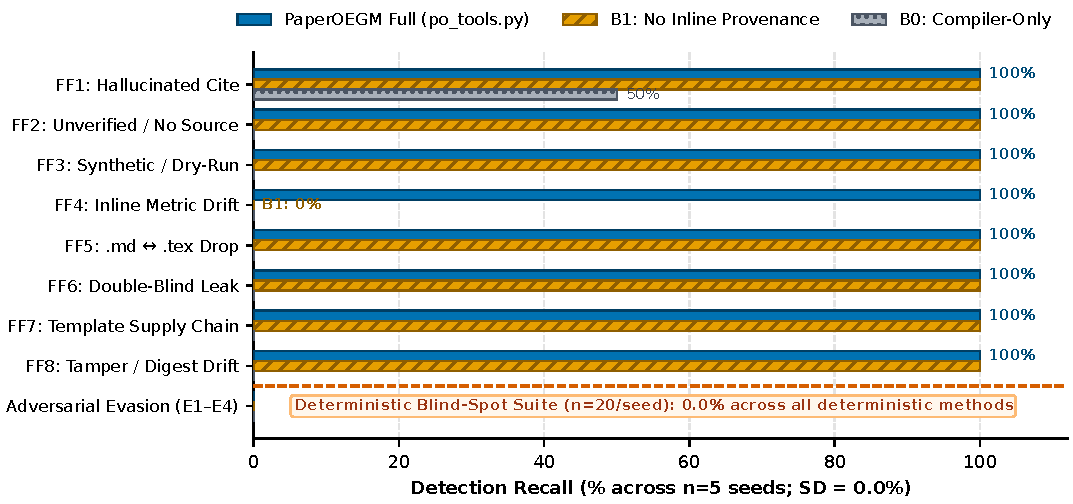
\includegraphics[width=0.88\textwidth]{figures/fig_faultbench_recall.pdf}
\caption{Per-family recall (\%) on PO-FaultBench (FF1--FF8, 80 positives + 40 negative controls/seed, $n=5$, SD $= 0.0\%$) and 20-case/seed adversarial evasion suite across PaperOEGM Full, B1 (No Inline Provenance), and B0 (Compiler-Only).}
\label{fig:faultbench}
\end{figure*}

\subsection{RQ2: Packaging, Context Footprint, and Determinism}\label{sec:exp-rq2}

\textbf{Setup.} Across five build runs (\texttt{42}--\texttt{46}), we compare PaperOEGM against \textbf{B2 (Monolithic Single-Skill)} concatenating all 10 skills, \texttt{execution\_\allowbreak{}instructions.\allowbreak{}md}, 6 protocols, and 5 review standards, and \textbf{B3 (Public EGM Reference)} measured on open-source \texttt{google/\allowbreak{}elephant-goldfish-model} v0.1.1 \citep{google2026egm} (scoped strictly to skill/agent footprint; non-applicable cells marked ---). We report whole-file \texttt{SKILL.\allowbreak{}md} bytes (decimal KB = 1,000 B for loader ceilings; binary KiB = 1,024 B for ZIP archives), active-stage load, startup frontmatter size, compliance defects \citep{zhang2026reusable}, live \texttt{claude\ plugin\ validate}, and deterministic ZIP SHA-256 parity across \texttt{antigravity}, \texttt{claude}, and \texttt{openai} via \texttt{scripts/\allowbreak{}pack\_\allowbreak{}plugin.\allowbreak{}py}.

\begin{table*}[t]
\centering
\footnotesize
\setlength{\tabcolsep}{4pt}
\caption{Multi-harness skill footprint, context reduction, compliance defects, and deterministic build parity ($n=5$ builds). Non-applicable baseline cells are marked ---; public EGM (B3) is scoped strictly to skill/agent footprint.}
\label{tab:packaging}
\begin{tabular}{lccccccc}
\toprule
\textbf{Packaging Strategy} & \textbf{Skills} & \textbf{Median / Max Skill (B)} & \textbf{Active Stage (B)} & \textbf{vs. Mono (\%)} & \textbf{Max Agent (B)} & \textbf{Defects} & \textbf{ZIP SHA-256} \\
\midrule
B2: Monolithic Single-Skill & 1 & 79,454 / 79,454 & 79,454 & 0.00\% & --- & --- & --- \\
B3: Public EGM Reference & 7 & 15,205 / 24,257 & --- & --- & 7,355 & --- & --- \\
\textbf{PaperOEGM (10 Skills)} & \textbf{10} & \textbf{3,900 / 4,526} & \textbf{14,171} & \textbf{-82.16\%} & \textbf{2,376} & \textbf{0} & \textbf{100.0\%} \\
\bottomrule
\end{tabular}
\end{table*}

\textbf{Results.} In Table~\ref{tab:packaging} and Figure~\ref{fig:footprint}, every PaperOEGM \texttt{SKILL.\allowbreak{}md} spans 3,466--4,526 bytes (median 3,900 B, maximum 63 lines)---preserving 62.28\% headroom below our 12 KB budget and 81.14\% below Antigravity's 24 KB (24,000 B) ceiling, whereas public EGM (B3) reaches 15,205 B median and 24,257 B max (+257 B over the 24,000 B limit; max agent 7,355 vs.~2,376 B). Protocol offloading reduces median active-stage context from 79,454 B (B2) to 14,171 B (-82.16\%; 15,749 B max stage) and startup index context to 2,270 B (-97.14\%). PaperOEGM yields 0 compliance defects, passes \texttt{claude\ plugin\ validate} cleanly, and produces byte-identical ZIPs (124.88 KiB Antigravity, 142.37 KiB Claude, 125.75 KiB OpenAI; 100.0\% SHA-256 parity) in 143.00 \(\pm\) 10.09 ms.

\begin{figure*}[t]
\centering
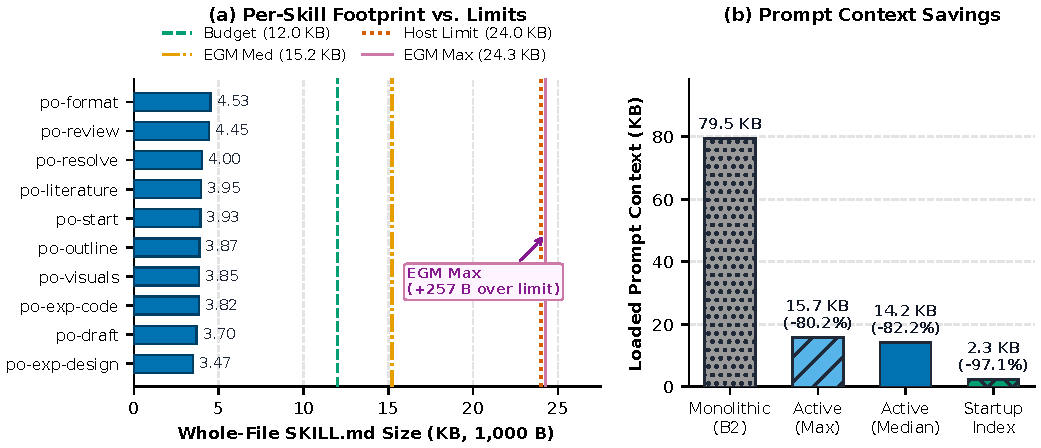
\includegraphics[width=0.88\textwidth]{figures/fig_skill_footprint.pdf}
\caption{Skill packaging footprint and context economics: (a) whole-file \texttt{SKILL.\allowbreak{}md} size (decimal KB, 1,000 B) across 10 PaperOEGM skills vs. 12 KB budget, public EGM v0.1.1 median/max (+257 B over ceiling), and Antigravity's 24 KB ceiling; (b) loaded prompt context across Monolithic (B2), active max/median, and startup index.}
\label{fig:footprint}
\end{figure*}

\subsection{RQ3: Scalability, Offloading, and Paranoid TeX Containment}\label{sec:exp-rq3}

\textbf{Setup.} We benchmark live subprocess runs of all four \texttt{po\_\allowbreak{}tools.\allowbreak{}py} subcommands across four scales over \(n=5\) seeds: \textbf{S} (20 cites, 5 runs), \textbf{M} (50/10), \textbf{L} (80/20), and \textbf{XL} (120/30), against a pre-experiment \texttt{\textless{}\ 250\ ms} XL target and \texttt{\textgreater{}\ 2,\allowbreak{}000\ ms} falsification bar. Each seed also runs two paranoid TeX suites (\texttt{openin\_\allowbreak{}any=p\ openout\_\allowbreak{}any=p\ pdflatex\ \mbox{-{}-}no-\allowbreak{}shell-escape}): (1) double-blind builds across \textbf{ACM SIGPLAN} (\texttt{acmart{[}sigplan,\allowbreak{}review,\allowbreak{}anonymous{]}}), \textbf{CVPR 2025}, and \textbf{ICLR 2025} audited via \texttt{pdfinfo} and \texttt{format-verify}; and (2) a \textbf{3-vector adversarial suite} executing E2 \texttt{\textbackslash{}csname\ write18\textbackslash{}endcsname}, parent \texttt{\textbackslash{}openout\ ../\allowbreak{}pwn\_\allowbreak{}out.\allowbreak{}txt}, and parent \texttt{\textbackslash{}openin\ ../\allowbreak{}secret\_\allowbreak{}parent.\allowbreak{}txt} (checked via \texttt{pdftotext}).

\textbf{Results.} Figure~\ref{fig:scalability}(a) shows 4-command latency staying flat from 266.00 \(\pm\) 7.28 ms (S) to 268.55 \(\pm\) 6.80 ms (XL; M: 265.49 \(\pm\) 4.94 ms, L: 262.39 \(\pm\) 7.84 ms; XL breakdown: \texttt{state-sync} 125.52 \(\pm\) 2.81, \texttt{check-readonly} 58.07 \(\pm\) 3.56, \texttt{review-preflight} 43.06 \(\pm\) 3.75, \texttt{format-verify} 41.91 \(\pm\) 3.51 ms). Figure~\ref{fig:scalability}(b) shows \texttt{literature/\allowbreak{}sources/} offloading saves 87.82\% (S) to 87.96\% (XL; 24,169 B loaded vs.~176,550 B offloaded). All 3/3 double-blind venues compile (\texttt{acmart{[}sigplan{]}} 1698.11 \(\pm\) 27.14 ms, \texttt{cvpr2025} 1285.42 \(\pm\) 28.64 ms, \texttt{iclr2025} 982.74 \(\pm\) 7.24 ms) with 0 identity leaks. On the adversarial suite, paranoid \texttt{pdflatex} blocks \textbf{2/3} exploits across all five seeds: E2 \texttt{\textbackslash{}csname\ write18\textbackslash{}endcsname} (1.0) and parent \texttt{\textbackslash{}openout} (1.0) are blocked, whereas parent \texttt{\textbackslash{}openin} read traversal is \textbf{not blocked} (0.0).

Three practical findings follow. First, XL latency (268.55 ms) slightly exceeded our 250 ms target (still \textgreater7\(\times\) below 2,000 ms) due to fixed cold Python startup across four processes; marginal 6\(\times\) scale growth is only +2.55 ms. Second, \texttt{cvpr2025}/\allowbreak{}\texttt{iclr2025} blank all three PDF identity fields, whereas \texttt{acmart} v2.16 injects a generic non-identifying \texttt{Creator:\ LaTeX\ with\ acmart\ ...} string via \texttt{hyperxmp} (1 generic tag, 0 identity leaks). Third, inspecting TeX Live 2026's \texttt{texmf.\allowbreak{}cnf} confirmed upstream TeX Live 2026 retired \texttt{openin\_\allowbreak{}any} into a silent no-op (always permitting input reads even when \texttt{kpsewhich} echoes \texttt{p}), proving untrusted templates require OS-level sandboxing (containers or \texttt{sandbox-exec}) alongside \texttt{\mbox{-{}-}no-\allowbreak{}shell-escape} and \texttt{openout\_\allowbreak{}any=p}.

\begin{figure*}[t]
\centering
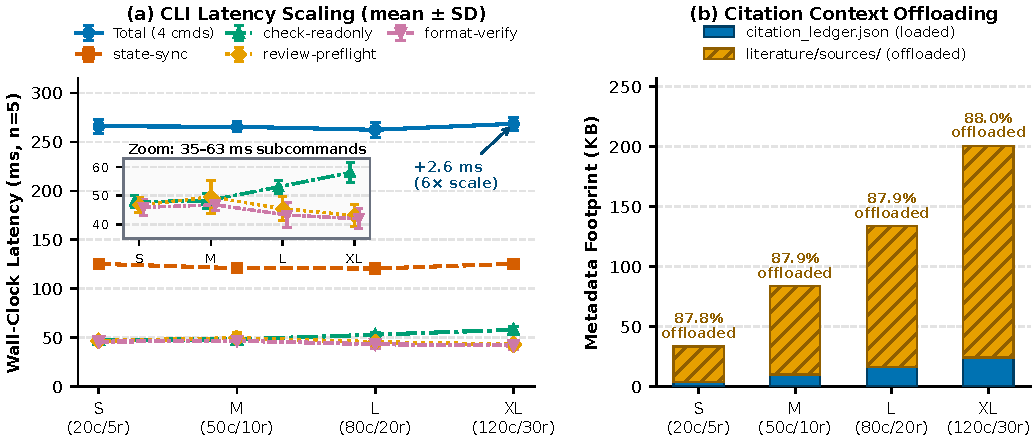
\includegraphics[width=0.88\textwidth]{figures/fig_scalability.pdf}
\caption{Verification scalability across S (20c/5r) to XL (120c/30r), $n=5$: (a) wall-clock CLI latency (mean $\pm$ SD) with 35--63 ms zoomed inset; (b) compact \texttt{citation\_\allowbreak{}ledger.\allowbreak{}json} vs. offloaded \texttt{literature/\allowbreak{}sources/} footprint (\% of total citation metadata offloaded).}
\label{fig:scalability}
\end{figure*}

\subsection{RQ4: Live Hybrid Fresh-Context Critic Audit}\label{sec:exp-rq4}

\textbf{Setup.} We construct \(n=3\) compact seeded mini-paper workspaces (\textasciitilde150--180 words across two sections each) spanning ML Systems (\texttt{s42}), Vision Benchmarks (\texttt{s43}), and Agent Security (\texttt{s44}). Each embeds 10 ground-truth defects stored outside the workspace: 5 mechanical (\textbf{M1} missing citation, \textbf{M2} unverified citation, \textbf{M3} decimal drift, \textbf{M4} synthetic/\texttt{dry\_\allowbreak{}run} leak, \textbf{M5} double-blind path/URL leak) and 5 semantic/evasion (\textbf{S1} \texttt{verified\_\allowbreak{}source} claim-vs-abstract distortion, \textbf{S2} integer-only count falsification, \textbf{S3} omitted ablation + overclaim + prose lab deanonymization, \textbf{S4} undefined math symbol + acronym, \textbf{S5} real \texttt{matplotlib} PNG rendered with colliding x-ticks, 4.5pt labels, missing units, and red-green bars). We run timed \texttt{po\_\allowbreak{}tools.\allowbreak{}py} (\texttt{review-preflight} + \texttt{format-verify}) as \textbf{B4 (Deterministic-Only)}, verify pre/post \texttt{check-readonly}, dispatch all five live read-only \texttt{po-*} critics flat in parallel on Antigravity (Gemini 4; 15 invocations), estimate output tokens via a whitespace proxy (\(\text{round}(\text{words}\times 1.3)\)), and track \texttt{clean\_\allowbreak{}control\_\allowbreak{}fp} on whether critics falsely flag the valid citation missing/unverified or the accurate secondary decimal mismatched.

\begin{table*}[t]
\centering
\footnotesize
\setlength{\tabcolsep}{4pt}
\caption{Live hybrid audit across $n=3$ compact seeded domain manuscripts (30 planted defects: 15 mechanical M1--M5, 15 semantic S1--S5; 15 live Antigravity read-only critic invocations; token counts via whitespace word-count proxy).}
\label{tab:hybrid}
\begin{tabular}{lcccccc}
\toprule
\textbf{Review Configuration} & \textbf{Mech. Recall (\%)} & \textbf{Sem. Recall (\%)} & \textbf{Total Recall (\%)} & \textbf{Clean FP} & \textbf{Mutations} & \textbf{Max Critic Tok.} \\
\midrule
B4: Deterministic-Only (\texttt{po\_\allowbreak{}tools.\allowbreak{}py}) & 100.0 $\pm$ 0.0 & 0.0 $\pm$ 0.0 & 50.0 $\pm$ 0.0 & 0.0 $\pm$ 0.0 & 0.0 & 0 \\
Fresh Read-Only Critics Alone (5 agents) & 100.0 $\pm$ 0.0 & 100.0 $\pm$ 0.0 & 100.0 $\pm$ 0.0 & 0.0 $\pm$ 0.0 & 0.0 & 1411.0 $\pm$ 35.68 \\
\textbf{PaperOEGM Hybrid (Full)} & \textbf{100.0 $\pm$ 0.0} & \textbf{100.0 $\pm$ 0.0} & \textbf{100.0 $\pm$ 0.0} & \textbf{0.0 $\pm$ 0.0} & \textbf{0.0} & \textbf{1411.0 $\pm$ 35.68} \\
\bottomrule
\end{tabular}
\end{table*}

\textbf{Results.} Table~\ref{tab:hybrid} shows B4 catching 100.0\% of M1--M5 in 91.71 \(\pm\) 0.26 ms at zero tokens but 0.0\% of S1--S5 (50.0\% total). Live flat-parallel critics recover 100.0\% of planted semantic flaws across all three domains (including multimodal inspection of \texttt{fig\_\allowbreak{}results.\allowbreak{}png} and integer count reconciliation), lifting recall to 100.0\% with 0.0 clean-control FPs, 0.0 workspace mutations, and all 15 runs within 1,500 tokens (mean peak 1411.0 \(\pm\) 35.68; \texttt{po-clarity-reader} 1400.33 \(\pm\) 48.81, \texttt{po-peer-reviewer} 1363.0 \(\pm\) 44.19, \texttt{po-visual-format-critic} 1108.33 \(\pm\) 64.78, \texttt{po-citation-auditor} 923.33 \(\pm\) 31.79, \texttt{po-evidence-auditor} 830.67 \(\pm\) 31.34).

Two scope qualifications apply. First, because critics also caught 100.0\% of M1--M5 on these compact drafts, RQ4 demonstrates \emph{one-way semantic lift} over B4 (0.0\% \(\to\) 100.0\%) rather than two-way recall separation; \texttt{po\_\allowbreak{}tools.\allowbreak{}py}'s necessity rests on RQ1/RQ3 (zero-stochasticity sub-110 ms checks at 120-citation scale and binary archive/SHA-256 audits impossible for shell-free read-only critics). Second, \texttt{po-citation-auditor} surfaced an unplanted template imprecision---flagging \texttt{"demonstrate\ strong\ baseline\ efficiency"} as unsupported by \texttt{wang2021tent} in \texttt{s43} (Nit) and contradicting \texttt{greshake2023indirect} in \texttt{s44} (Major)---confirming snapshot-grounded critique while illustrating that targeted \texttt{clean\_\allowbreak{}control\_\allowbreak{}fp} does not measure all unplanted findings.

\section{Limitations and Threats to Validity}\label{sec:limitations}

We highlight six candid limitations and threats to validity.

\textbf{Self-Benchmark Circularity and Deterministic Scope (RQ1).} Because \texttt{po\_\allowbreak{}tools.\allowbreak{}py} and PO-FaultBench were co-authored, 100.0\% recall and 0.0\% FPR on FF1--FF8 verify adherence to PaperOEGM's schema rather than universal error detection, and four families target PaperOEGM-specific files. Unordered set matching in Equation~\eqref{eq:decimal-match} also cannot detect metric-key swaps, unit-ambiguous \([0, 1]\) scaling, or untagged paragraphs. Our 20-case evasion suite (0.0\% recall) makes these boundaries explicit; external evaluation on PaperBench \citep{starace2025paperbench} or historical errata remains future work.

\textbf{TeX Read-Sandbox Regression and Prompt Injection (RQ3).} Static regexes miss macro-obfuscated TeX escapes (0.0\% recall on E2). While RQ3 confirmed \texttt{\mbox{-{}-}no-\allowbreak{}shell-escape} and \texttt{openout\_\allowbreak{}any=p} block \texttt{\textbackslash{}csname\ write18\textbackslash{}endcsname} (1.0) and parent \texttt{\textbackslash{}openout} writes (1.0), upstream TeX Live 2026 made \texttt{openin\_\allowbreak{}any=p} a silent no-op (0.0 blocked on parent \texttt{\textbackslash{}openin} reads), requiring OS-level containers or \texttt{sandbox-exec} for read isolation. Furthermore, although \citet{schmotz2026skillinject} report up to 80\% ASR for skill-file prompt injections, we did not empirically test adaptive indirect prompt injection inside scraped abstracts or PDFs against our read-only critics; read-only isolation bounds write blast radius but does not prevent finding suppression.

\textbf{RQ4 Scope and Missing Baselines.} Under zero external API keys, RQ4 evaluates \(n=3\) compact (\textasciitilde150--180 word) seeded drafts on one host/model (Antigravity / Gemini 4) without a same-context self-review or single-agent critic ablation. Achieving 100.0\% recall reflects dense planted flaws on short drafts; subtler defects on 9-page papers with 80+ citations will incur lower recall, consistent with the findings of \citet{liang2024feedback}, and \texttt{clean\_\allowbreak{}control\_\allowbreak{}fp} inspects targeted tokens rather than a defect-free manuscript.

\textbf{Asymmetric Cross-Harness Verification.} Antigravity (all 10 skills and 5 live critics) and Claude Code CLI packaging (\texttt{claude\ plugin\ validate} and install) were live-verified; Codex support is structurally verified via manifests and deterministic ZIP builds, not yet live-executed.

\textbf{Dogfooding Friction Points.} Self-hosting exposed four minor trade-offs: four separate \texttt{po\_\allowbreak{}tools.\allowbreak{}py} process launches incur \textasciitilde266 ms startup overhead (\texttt{266.00}--\texttt{268.55\ ms}); \texttt{acmart} v2.16 writes a generic non-identifying \texttt{Creator} via \texttt{hyperxmp}; literal path/marker mentions in meta-papers describing PaperOEGM can trip substring guards; and \texttt{check-readonly} tracks macOS \texttt{.DS\_\allowbreak{}Store} metadata unless excluded.

\textbf{Human Accountability.} PaperOEGM is strictly a human-in-the-loop aid (\texttt{disable-model-invocation:\ true}), not an autonomous paper mill; researchers remain responsible for scientific validity, Institutional Review Board (IRB) compliance, real experiments, and final verification.

\section{Conclusion}\label{sec:conclusion}

Reliable Agent Skills for scientific authoring require moving beyond monolithic playbooks and same-context LLM self-review. We presented \textbf{PaperOEGM}, a zero-API-key plugin packaged for Antigravity (live-verified end to end), Claude Code (packaging-validated), and Codex (structurally packaged), combining ten progressive-disclosure skills, a zero-dependency standard-library verifier (\texttt{po\_\allowbreak{}tools.\allowbreak{}py}), five flat single-level read-only critics, and paranoid LaTeX compilation.

Our evaluation yields three lessons for Agent Skills designers:

\begin{enumerate}
\def\labelenumi{\arabic{enumi}.}
\item
  \textbf{Strict byte budgets unlock portability:} Capping each \texttt{SKILL.\allowbreak{}md} at 12 KB (3,466--4,526 B actual, at most 63 lines) cuts median active-stage prompt context by 82.16\% and startup index load by 97.14\%, keeps 81.14\% headroom below Antigravity's 24 KB limit (exceeded by public EGM at 24,257 B), and achieves 100.0\% ZIP SHA-256 parity with 0 defects.
\item
  \textbf{Deterministic scripts, native sandboxes, and semantic critics are complementary:} \texttt{po\_\allowbreak{}tools.\allowbreak{}py} catches 100.0\% of mechanical faults on PO-FaultBench with 0.0\% FPR in 108.20 ms/workspace and scales to 120 citations in 268.55 ms (87.96\% ledger offloading; 3/3 double-blind venues, 0 identity leaks), yet records 0.0\% recall on semantic and macro evasions. Pairing deterministic checks with flat read-only critics recovers 100.0\% of planted semantic flaws (0 mutations, bounded tokens), while adversarial TeX testing proved \texttt{\mbox{-{}-}no-\allowbreak{}shell-escape} and \texttt{openout\_\allowbreak{}any=p} hold even as TeX Live 2026 retired \texttt{openin\_\allowbreak{}any=p}.
\item
  \textbf{Zero-API-key design eases adoption:} Relying only on the host coding runtime and Python's standard library (plus optional \texttt{matplotlib} for Stage 5 plots) removes credential coupling and dependency drift.
\end{enumerate}

Future work includes OS-level container/sandbox wrappers for TeX read isolation on TeX Live 2026+, cross-harness live critic benchmarks (with same-context and single-agent baselines) on Claude Code and Codex, batched single-process \texttt{po\_\allowbreak{}tools.\allowbreak{}py} execution, Abstract Syntax Tree (AST)-level TeX macro auditing, \texttt{.DS\_\allowbreak{}Store} exclusion in \texttt{check-readonly}, and community expansion of PO-FaultBench.


{\interlinepenalty=10000
\bibliographystyle{ACM-Reference-Format}
\bibliography{references}}

\end{document}
